
\begin{table}[t]
	%\centering
	%\tiny 
	\scriptsize
	\caption{Workload parameters.}
	\resizebox{\columnwidth}{!}{%
	\begin{tabular}{| c | c | c | c | c | c | c | c |} 
		\hline
	\textbf{Trace}    &   \textbf{\#GET L} & \textbf{\#GET M} & \textbf{\#PUT L} & \textbf{\#PUT M} & \textbf{\#Uniq L} & \textbf{\#Uniq M} \\ 
		\hline\hline
		\textbf{Dal}    &  2867  & 2000   & 124  & 9     & 1278 & 88      \\ 
		\hline
		\textbf{Fra}     &  1602  & 3278   & 111  & 9     & 420 & 43     \\
		\hline
		\textbf{Lon}    &  924    & 3972   & 98  & 6      & 698 & 88    \\
		\hline 
		\textbf{Syd}      &  1310   & 3653   & 35 & 2     & 154 & 18      \\  
		\hline
	\end{tabular}}

\label{tab:eval-overall}
\end{table}


%\begin{table}[h!]
%	%\centering
%	\scriptsize 
%	\caption{Testing Dataset.}
%	\begin{tabular}{| c | c | c | c | c | } 
%		\hline
%		Trace  (GB)  &   Dataset  & Data transferred  & GET L size  & PUT L size  \\ 
%		\hline\hline
%		Dal   & 20  & 37 & 35 & 2    \\ 
%		\hline
%		Fra     & 6  & 16 & 14 & 2   \\
%		\hline
%		Lon    &10   &  14 &12  & 2      \\
%		\hline 
%		Syd      &  2  &  9 & 8 & 1      \\  
%		\hline
%	\end{tabular}
%	
%	\label{tab:eval-dataset}
%\end{table}


%\begin{figure}[t]
%	\centering
%	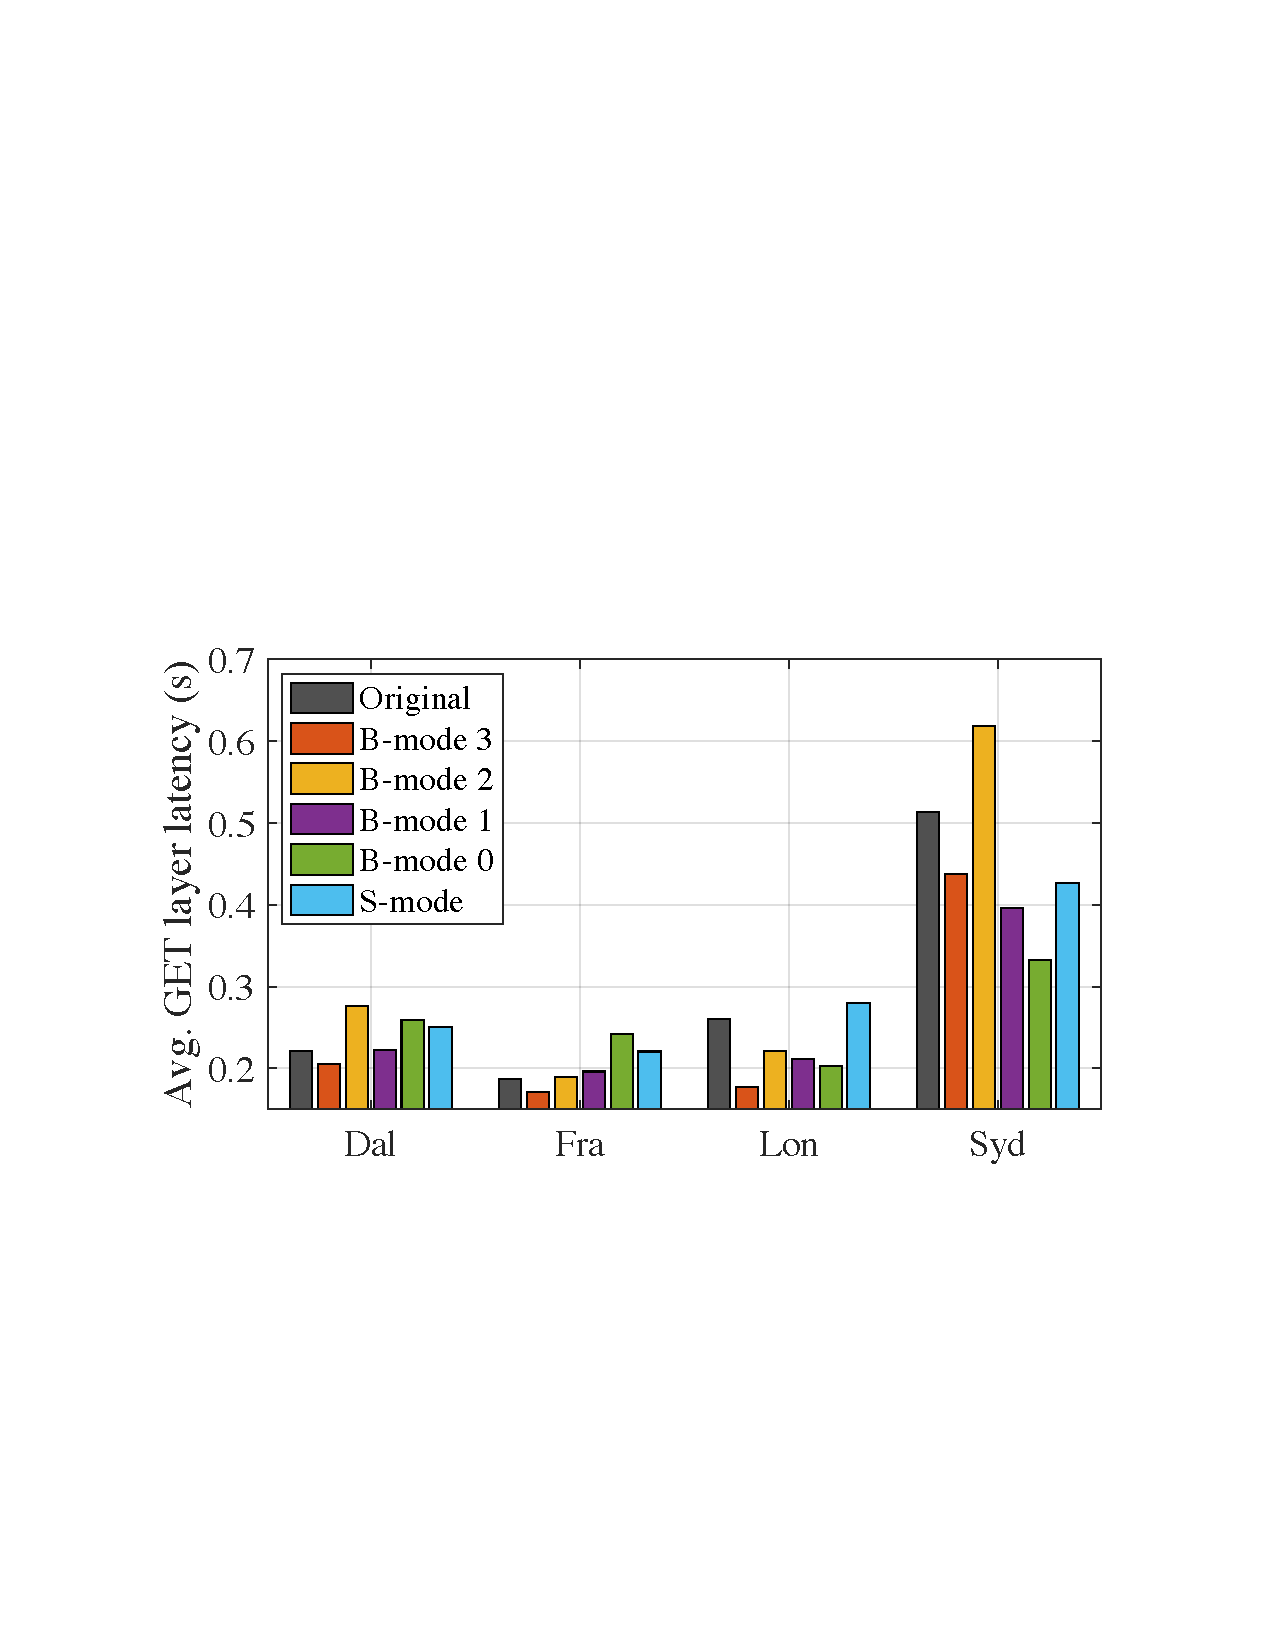
\includegraphics[width=0.45\textwidth]{graphs/get-layer-latency.pdf}
%	\caption{GET layer latency across different workloads from different schemes.}
%	%	\vspace{-3pt}
%	\label{fig:getlayerlatency}
%	
%\end{figure}

